%!TEX program = xelatex
\documentclass[11pt,a4paper]{article}
\usepackage[utf8]{inputenc}
\usepackage[T1]{fontenc}
\usepackage{authblk}
\usepackage{ctex}
\usepackage{tikz}
\usepackage{pgfplots}
\usepackage{verbatim}
\usepackage{amsfonts}
\usepackage{amsmath}
\usepackage{amsthm}
\usepackage{indentfirst}
\usepackage{amssymb}
\setlength{\parindent}{0pt}
\usetikzlibrary{shapes,snakes}
\newcommand{\argmax}{\operatornamewithlimits{argmax}}
\newcommand{\argmin}{\operatornamewithlimits{argmin}}
\DeclareMathOperator{\col}{col}
\usepackage{booktabs}
\newtheorem{theorem}{Theorem}
\newtheorem{note}{Note}
\newtheorem{definition}{Definition}
\newtheorem{proposition}{Proposition}
\newtheorem{lemma}{Lemma}
\newtheorem{example}{Example}
\newtheorem{corollary}{Corollary}
\usepackage{graphicx}
\usepackage{geometry}
\usepackage{hyperref}
\newcommand{\code}{	exttt}
\geometry{a4paper,scale=0.8}
\title{STAT 425 Note 2}
\author[*]{Wenxiao Yang}
\affil[*]{Department of Mathematics, University of Illinois at Urbana-Champaign}
\date{2021}

\usepackage{listings}
\usepackage{xcolor}

\lstset{numbers=left,numberstyle=\tiny,keywordstyle=\color{blue},commentstyle=\color[cmyk]{1,0,1,0},frame=single,escapeinside=``,extendedchars=false,xleftmargin=2em,xrightmargin=2em,aboveskip=1em,tabsize=4,showspaces=false}






\begin{document}
\maketitle
\tableofcontents
\newpage




\section{Generalized Least Squares}
What do we do if the errors are \textbf{correlated} or \textbf{heteroscedastic}?\\
Suppose $\varepsilon \sim \mathcal{N}_{n}(0, \Sigma)$, where $\Sigma$ is the variance-covariance matrix.
\subsection{GLS, $\Sigma$ known ($\hat{\beta}=\left(\mathbf{X}^{\top} \Sigma^{-1} \mathbf{X}\right)^{-1} \mathbf{X}^{\top} \Sigma^{-1} \mathbf{y}$, ${RSS}=(\mathbf{y}-\mathbf{X} \beta)^{\top} \Sigma^{-1}(\mathbf{y}-\mathbf{X} \beta)$)}
\subsubsection{Method 1: Transform back to OLS}
$$
\mathbf{y}=\mathbf{X} \beta+\varepsilon
$$
where $\varepsilon \sim \mathcal{N}_{n}(0, \Sigma)$ and $\Sigma$ is a known, symmetric, positive definite covariance matrix.\\
When the errors are heteroscedastic or correlated:\\
Transform this problem back to Ordinary Least-Squares (OLS):\\
1. Assume $S^{-1}$ exists and write
$$
\Sigma=S S^{\top}
$$
(We could use, for example, the Cholesky decomposition from linear algebra to obtain $S$.)\\

2. Multiply the model equation by $S^{−1}$ on both sides:
$$
\begin{aligned}
\mathbf{y} &=\mathbf{X} \beta+\varepsilon \\
S^{-1} \mathbf{y} &=S^{-1}(\mathbf{X} \beta+\varepsilon) \\
\underbrace{S^{-1} \mathbf{y}}_{:=\mathbf{y}^{*}} &=\underbrace{S^{-1} \mathbf{X}}_{:=\mathbf{x}^{*}} \beta+\underbrace{S^{-1} \varepsilon}_{:=\varepsilon^{*}} \\
\mathbf{y}^{*} &=\mathbf{X}^{*} \beta+\varepsilon^{*}
\end{aligned}
$$
This implies that
$$
\varepsilon^{*} \sim \mathcal{N}(S^{-1} \mathbf{0}, \underbrace{S^{-1} \Sigma\left(S^{-1}\right)^{\top}}_{=\text {ldentity }})=\mathcal{N}(\mathbf{0}, \mathbf{I})
$$
since $S^{-1} \Sigma\left(S^{-1}\right)^{\top}=S^{-1} S S^{\top}\left(S^{-1}\right)^{\top}=I$\\

3. For the transformed model, we can solve for $\beta$ using OLS:
$$
\mathbf{y}^{*}=\mathbf{X}^{*} \beta+\varepsilon^{*}
$$
where $\mathbf{y}^{*}=S^{-1} \mathbf{y}, \mathbf{X}^{*}=S^{-1} \mathbf{X}$\\
So, the estimator for $\beta$ computes as
$$
\begin{aligned}
\hat{\beta} &=\left(\mathbf{X}^{* \top} \mathbf{X}^{*}\right)^{-1} \mathbf{X}^{* \top} \mathbf{y}^{*} \\
&=(\mathbf{X}^{\top} \underbrace{\left(S^{-1}\right)^{\top} S^{-1}}_{=\Sigma^{-1}} \mathbf{X})^{-1} \mathbf{X}^{\top} \underbrace{\left(S^{-1}\right)^{\top} S^{-1}}_{=\Sigma^{-1}} \mathbf{y} \\
&=\left(\mathbf{X}^{\top} \Sigma^{-1} \mathbf{X}\right)^{-1} \mathbf{X}^{\top} \Sigma^{-1} \mathbf{y}
\end{aligned}
$$
Note that the solution we obtained minimizes:
$$
\left\|\mathbf{y}^{*}-\mathbf{X}^{*} \beta\right\|^{2}=(\mathbf{y}-\mathbf{X} \beta)^{\top} \Sigma^{-1}(\mathbf{y}-\mathbf{X} \beta)
$$

\subsubsection{Weighted Least Squares (WLS)}
Suppose that $\Sigma$ is a diagonal matrix of unequal error variances:
$$
\Sigma=\operatorname{diag}\left(\sigma_{1}^{2}, \sigma_{2}^{2}, \ldots, \sigma_{n}^{2}\right)
$$
The GLS estimate of $\beta$ minimizes:
$$
(\mathbf{y}-\mathbf{X} \beta)^{\top} \Sigma^{-1}(\mathbf{y}-\mathbf{X} \beta)=\sum_{i=1}^{n} \frac{\left(y_{i}-\mathbf{x}_{i}^{\top} \beta\right)^{2}}{\sigma_{i}^{2}}
$$
This problem is known as the Weighted Least-Squares (WLS).\\
Note that the errors are weighted by
$$
w_{i}=\frac{1}{\sigma_{i}^{2}}
$$
smaller weights for samples with larger variances.

\subsubsection{WLS special example : Replicated Observations}
Suppose we collected multiple observations for each $\mathbf{x}_{i}$. We use double subscripts to indicate the replicate observations:
$$
\left(\mathbf{x}_{i}, y_{i 1}, y_{i 2}, \ldots, y_{i n_{i}}\right)
$$
Let $y_{i}$ denote the average of the $n_{i}$ observations sharing $\mathbf{x}_{i}$. Then the residual sum of squares for $\beta$ equals
$$
\sum_{i=1}^{n} \sum_{j=1}^{n_{i}}\left(y_{i j}-\mathbf{x}_{i}^{\top} \beta\right)^{2}=\sum_{i=1}^{n} n_{i}\left(y_{i}-\mathbf{x}_{i}^{\top} \beta\right)^{2}+\sum_{i=1}^{n} \sum_{j=1}^{n_{i}}\left(y_{i j}-y_{i}\right)^{2}
$$
Minimizing the $RSS$ to solve for $\beta$ is the same as minimizing the first term on the right only.
$$\hat{\beta}=\argmin_\beta \sum_{i=1}^n n_i(y_i-\mathbf{x}_i^T\beta)^2$$

\subsubsection{Method 2: Likelihood Estimation}
Model: $\mathbf{y} \sim N_{n}(\mathbf{X} \beta, \Sigma)$\\
Log-likelihood:
$$
\begin{aligned}
&\log (p(\mathbf{y} \mid \beta, \Sigma)) \\
&\quad=\log \left\{\frac{1}{(2 \pi)^{n / 2}|\Sigma|^{1 / 2}} \exp \left[-\frac{1}{2}(\mathbf{y}-\mathbf{X} \beta)^{\top} \Sigma^{-1}(\mathbf{y}-\mathbf{X} \beta)\right]\right\} \\
&\quad=-\frac{1}{2}(\mathbf{y}-\mathbf{X} \beta)^{\top} \boldsymbol{\Sigma}^{-1}(\mathbf{y}-\mathbf{X} \beta)+\text { Constant. }
\end{aligned}
$$
Therefore the MLE is given by
$$
\hat{\beta}_{m l e}=\arg \min _{\beta}(\mathbf{y}-\mathbf{X} \beta)^{\top} \Sigma^{-1}(\mathbf{y}-\mathbf{X} \beta)
$$

\subsection{GLS, $\Sigma$ unknown}
\subsubsection{Method 1: Estimation of Variance ($r_i^2$)/Standard Deviation Function ($|r_i|$)}
$$\sigma_i^2=\mathbb{E}(\varepsilon_i^2)-(\mathbb{E}(\varepsilon_i))^2$$
Since we assume $E(\varepsilon_i)=0$, we have
$$\sigma_i^2=\mathbb{E}(\varepsilon_i^2)$$
Which implies $r_i^2$ is an estimator of $\sigma_i^2$; $|r_i|$ is an estimator of the standard deviation $\sigma_i$.\\

\textbf{Estimate Variance Function} $\hat{v_i}(x)$

1. Fit a regression model using OLS, and obtain the residuals $r_i$.\\
2. Regress the squared residuals $r_i^2$ against the appropriate predictor variables.\\
Denote $\hat{v_i}$ be the fitted value from variance function
$$w_i=\frac{1}{\hat{v_i}}$$

\textbf{Estimate Standard Deviation Function} $\hat{s_i}(x)$

1. Fit a regression model using OLS, and obtain the residuals $r_i$.\\
2. Regress the absolute residuals $|r_i|$ against the appropriate predictor variables.\\
Denote $\hat{s_i}$ be the fitted value from standard deviation function
$$w_i=\frac{1}{(\hat{s_i})^2}$$
The estimated variances are then placed in the variance-covariance matrix $\Sigma$ and the regression coefficients are estimated using the WLS (Weighted Least Squares method).

\subsubsection{Method 2: iterative approach}
1. Start with some initial guess of $\Sigma$\\
2. Use $\Sigma$ to estimate $\beta$\\
3. Use residuals (since we have known $\beta$) to estimate $\Sigma$\\
4. Iterate until convergence.\\

It looks like a good idea; however the methods will not work if we do not assume some structure about $\Sigma$ (too many parameters to be estimated).

Based on the application, we can assume a particular structure for $\Sigma$ that does not involve too many parameters.\\
Then, we can model $\beta$ and $\Sigma$ simultaneously.\\
For example , for AR(1) times series (auto-regressive model of order 1),
the structure of $\Sigma$ would be:
$$\Sigma=\sigma^2 \begin{pmatrix}
    1& \rho& \rho^2& \rho^3& \cdots\\
    \rho& 1& \rho& \rho^2& \cdots \\
    \cdots & \cdots& \cdots &\cdots&\cdots \\
    \rho^{n-1}& \rho^{n-2}&\cdots&\cdots&1
\end{pmatrix}$$
$\Sigma$ as a function of $\rho$ and $\sigma^2$.

\section{Lack of Fit Tests}
\subsection{Gaussian Assumption}
Gaussian Assumption, which can be summarized concisely as:
$$y\sim \mathcal{N}_{n}(\mathbf{X}\beta, \sigma^2 \mathbf{I})$$
Under these assumptions:
\begin{equation}
    \begin{aligned}
        \hat{\beta}&=\left(\mathbf{X}^{T} \mathbf{X}\right)^{-1} \mathbf{X}^{T} y\sim \mathcal{N}_{p}(\beta,\sigma^2\left(\mathbf{X}^{T} \mathbf{X}\right)^{-1}),\\
        \hat{y}&=\mathbf{X}\hat{\beta}\sim \mathcal{N}_{n}(\mathbf{X}\beta, \sigma^2 \mathbf{H})
    \end{aligned}
    \nonumber
\end{equation}
independently,
$$\hat{\sigma}^2=\frac{RSS}{n-p}=\frac{||y-\hat{y}||^2}{n-p}\sim \sigma^2\frac{\chi^2_{n-p}}{n-p}$$

\subsection{When $\sigma^2$ is known}
Intuition:\\
If the model is correct, then $\hat{\sigma}^2$ is an unbiased estimate of $\sigma^2$.\\
If we know $\sigma^2$, we could construct a test based on the ratio $\frac{\hat{\sigma}^2}{\sigma^2}$, a measure of \textit{lack-of-fit}.

In this case we want to test the hypothesis:
$$
\left\{\begin{array}{l}
H_{0}: \text { There is no lack of fit. } \\
H_{\alpha}: \text { There is lack of fit. }
\end{array}\right.
$$
We use the test statistic:
$$
\frac{\hat{\sigma}^{2}}{\sigma^{2}}=\frac{R S S /(n-p)}{\sigma^{2}} \sim \frac{\chi_{n-p}^{2}}{n-p}
$$
Lack of fit means the error variance is large related to the value of $\sigma^{2}$, i.e., the test statistic is large.\\
Conclude that there is lack of fit (i.e. Reject $\left.H_{0}\right)$, if:
$$
(n-p) \frac{\hat{\sigma}^{2}}{\sigma^{2}} \geq \chi_{n-p}^{2}(1-\alpha)
$$

\subsection{When $\sigma^2$ is unknown}
\subsubsection{Hypothesis}
If $\sigma^{2}$ is unknown, a general approach is to compare an estimate of $\sigma^{2}$ based on a \underline{much bigger/general model}.\\
If we can derive the distribution (under $\mathrm{H}_{0}$ ) of $\hat{\sigma}_{\text {LinearModel }}^{2} / \hat{\sigma}_{\text {BigModel }}^{2}$, then we reduce this problem to a two model comparison test problem.\\
The null hypothesis is the current model:\\
$H_{0}: \mathbb{E}\left(y_{i}\right)=\mathbf{x}_{i}^{\top} \beta, \quad i=1,2, \ldots, n, \quad$ for some vector $\beta$\\
The more general model is assumed under the alternative hypothesis:\\
$H_{\alpha}: \mathbb{E}\left(y_{i}\right)=f\left(\mathbf{x}_{i}\right), \quad i=1,2, \ldots, n$, \quad for some function $f$\\

\subsubsection{Under the null hypothesis $H_{0}$}
$y_{i j}=\mathbf{x}_{i}^{\top} \beta+\varepsilon_{i j}$, some $\beta, \varepsilon_{i j} \sim$ iid $\mathcal{N}\left(0, \sigma^{2}\right)$\\
$R S S_{0}$ with $d f=n-p$
\subsubsection{Under the alternative big-model hypothesis $H_{\alpha}$ :}
$y_{i j}=f\left(\mathbf{x}_{i}\right)+\varepsilon_{i j}$, some function $f, \varepsilon_{i j} \sim$ iid $\mathcal{N}\left(0, \sigma^{2}\right)$\\
\textbf{Can we estimate $\sigma^{2}$ for the big model in $H_{\alpha}$ ?}\\
- The answer is yes, if there is some replication in the data, i.e., there are multiple observations (replicates) for some (at least) of the same $\mathbf{x}_{i}$ values.\\
- Schematically we can represent these replicates as:
$$
\left(\mathbf{x}_{i}, y_{i 1}, y_{i 2}, \ldots, y_{i n_{i}}\right), \quad i=1: m, \quad n=\sum_{i} n_{i}
$$
$R S S_{a}$ with $d f=n-m=\sum_{i}\left(n_{i}-1\right)$, where
$$
R S S_{a}=\sum_{i=1}^{m} \sum_{j=1}^{n_{i}}\left(y_{i j}-\bar{y}_{i .}\right)^{2}
$$
\subsubsection{$F-$Test}
All of the degrees of freedom for $R S S_{a}$ come from the replications. Therefore, with replication we can do an $\mathrm{F}$ test for lack of fit:
$$
F=\frac{\left(R S S_{0}-R S S_{a}\right) /(m-p)}{R S S_{a} /(n-m)} \sim F_{m-p, n-m}
$$

\section{Polynomials Regression}
\subsection{Basic Function}
\begin{equation}
    \begin{aligned}
        y_i&=f(x_i)+\varepsilon_i\\
        y_i&=\beta_0+\sum_{j=1}^db_j(x_i)\beta_j+\varepsilon_i\\
        y_i&=\beta_0+\sum_{j=1}^d\beta_j
        x_i^j+\varepsilon_i\\
    \end{aligned}
    \nonumber
\end{equation}
$d$ is the \textbf{degree of the polynomial component}.\\
\subsection{Choose Order $d$}
1.\textbf{Forward Approach}: Keep adding terms until the last added term is not significant.\\
2.\textbf{Backward Approach}: Start with a large $d$, and keep eliminating the terms that are not statistically significant, starting with the highest order term.\\

Once we pick up a $d$, we do not test the significance of the lower-order terms. (include all the lower-order terms in our model by default)\\
\textbf{Reasoning}: we do not want our results to be affected by a change of location/scale of the data. $(z_i-2)^2=z_i^2-4z_i+4$.\\
\textbf{Exception}: particular polynomial function (physics law).


\subsection{Orthogonal Polynomials}
Successive predictors $x^j$ are \textbf{highly correlated} introducing multicollinearity problems.
\begin{equation}
    \begin{aligned}
        y_i=\beta_0+\beta_1 \mathbf{z}_i+...+\beta_d \mathbf{z}_d+\varepsilon_i
    \end{aligned}
    \nonumber
\end{equation}
where $\mathbf{z}_j=a_1+b_2x+...+\kappa_j x^j$ is a polynomial of order $j$ with coefficients chosen such that $\mathbf{z}_j^T\mathbf{z}_j=0$

\subsection{Piece-wise Polynomials}
If the true mean of $E(Y | X = x) = f (x)$ is too wiggly, we might need to fit a higher order polynomial, which is not always a good idea.\\

Instead we will consider \textbf{piece-wise polynomials}:

1.we divide the range of $x$ into several intervals, and

2.within each interval $f (x)$ is a low-order polynomial, e.g., cubic or quadratic, but the polynomial coefficients change from interval to interval;

3.in addition we require the overall $f (x)$ to be continuous up to certain derivatives.

\subsection{Cubic Splines}
\subsubsection{Why Spline}
\textbf{Polynomials}: smooth, but each point affects the fit globally.\\
\textbf{Piece-wise Polynomials}: localizes the influence of each data point, but are not smooth enough.\\
\textbf{Splines}: combines the beneficail aspects of both approaches.\\

\subsubsection{Settings}
A \textbf{Cubic Spline} is a curve constructed from sections of cubic polynomials, joined together so that the curve is \textit{continuous up to second derivative}.\\
The points at which the sections join are called the \textbf{knots} of the spline.\\

We want to define a cubic spline function in the interval $[a, b]$\\
- Define $m$ knots such that: $a<\xi_{1}<\xi_{2}<\ldots<\xi_{m}<b$\\
- A function $g$ defined on $[a, b]$ is a \textbf{cubic spline with respect to knots $\left\{\xi_{i}\right\}_{i=1}^{m}$} if:\\
1. $g$ is a cubic polynomial in each of the $m+1$ intervals,
$$
g(x)=d_{i} x^{3}+c_{i} x^{2}+b_{i} x+a_{i}, \quad x \in\left[\xi_{i}, \xi_{i+1}\right]
$$
where $i=0, \ldots, m, \xi_{0}=a$ and $\xi_{m+1}=b$\\
2. $g$ is continuous up to the 2 nd derivative: since $g$ is continuous up to the 2nd derivative for any point inside an interval, it suffices to check the following conditions:
$$
g^{(0,1,2)}\left(\xi_{i}^{+}\right)=g^{(0,1,2)}\left(\xi_{i}^{-}\right), \quad i=1: m
$$
This expression indicates that the function and the first and second order derivatives are continuous at the knots.\\

\subsubsection{Number of free parameters: $m+4$}
How many free parameters do we need to represent a cubic spline?\\
(i) 4 parameters $\left(d_{i}, c_{i}, b_{i}, a_{i}\right)$ for each of the $(m+1)$ intervals.\\
(ii) 3 constraints at each of the $m$ knots (continuity constraints).\\
The \textbf{total number of free parameters} (similar to the number of degrees of freedom) is:
$$
4(m+1)-3 m=m+4
$$

\subsubsection{Properties: linear combination also cubic spline}
Given knots $\{\xi_i\}_{i=1}^m$, the linear combinations of cubic splines are also cubic splines.\\
That is, for a set of given knots, the corresponding cubic splines form a linear space (of functions) with ${dim} (m + 4)$.

\subsubsection{Cubic Splines Basis}
A set of basis functions for cubic splines (w.r.t knots $\left\{\xi_{i}\right\}_{i=1}^{m}$ ) is given by:
$$
\begin{aligned}
h_{0}(x) &=1 \\
h_{1}(x) &=x \\
h_{2}(x) &=x^{2} \\
h_{3}(x) &=x^{3} \\
h_{i+3}(x) &=\left(x-\xi_{i}\right)_{+}^{3}, \quad i=1,2, \ldots, m
\end{aligned}
$$
That is, any cubic spline can be uniquely expressed as:
$$
\beta_{0}+\sum_{j=1}^{m+3} \beta_{j} h_{j}(x)
$$
Given knot locations, there are many alternative, but equivalent ways of writing down a basis for cubic splines.
\begin{example}[Other Basis]
    For example, another basis for cubic splines can be the following:
    $$
    \begin{aligned}
    h_{0}(x) &=1 \\
    h_{1}(x) &=x \\
    h_{i+1}(x) &=R\left(x, \xi_{i}^{*}\right), i=1, \ldots, q-1
    \end{aligned}
    $$
    where
    $$
    \begin{aligned}
    R(x, z)=&\left[(z-1 / 2)^{2}-1 / 12\right]\left[(x-1 / 2)^{2}-1 / 12\right] / 4 \\
    &-\left[(|x-z|-1 / 2)^{4}-1 / 2(|x-z|-1 / 2)^{2}+7 / 240\right] / 24
    \end{aligned}
    $$
\end{example}

\subsection{Natural Cubic Splines (NCS)}
A cubic spline on $[a, b]$ is a \textbf{Natural Cubic Spline} if its \textit{second and third derivatives are zero at a and $b$}.
\subsubsection{Degree of Freedom (Number of free parameters): $m$}
This condition implies that NCS is a linear function in the two extreme intervals $\left[a, \xi_{1}\right]$ and $\left[\xi_{m}, b\right]$. The linear functions in the two extreme intervals are completely determined by their neighboring intervals.\\
The degree of freedom of NCS's with $m$ knots is:
$$
4(m+1)-3 m-4=m
$$
(We have 4 additional constraints.)

\subsubsection{NCS Basis}
A Natural Cubic Spline with $m$ knots is represented by $m$ basis functions, for example, one such basis is given by
$$
\begin{aligned}
N_{1}(x) &=1 \\
N_{2}(x) &=x \\
N_{k+2}(x) &=d_{k}(x)-d_{k-1}(x)
\end{aligned}
$$
where
$$
d_{k}(x)=\frac{\left(x-\xi_{k}\right)_{+}^{3}-\left(x-\xi_{m}\right)_{+}^{3}}{\xi_{m}-\xi_{k}}
$$
Each of these derivatives can be seen to have zero second and third derivative for $x \geq \xi_{m}$.

\subsubsection{Note: Waste of Data points}
Recall that the \textbf{linear functions} in the two extreme intervals are completely determined by the other cubic splines. So data points in the two extreme intervals (i.e., outside the two boundary knots) are wasted since they do not affect the fitting.\\











\subsection{Regression Splines}
We can represent the model on the observed $n$ data points using matrix notation:
$$
\left(\begin{array}{l}
y_{1} \\
y_{2} \\
\ldots \\
y_{n}
\end{array}\right)_{n \times 1}=\left(\begin{array}{llll}
h_{0}\left(x_{1}\right) & h_{1}\left(x_{1}\right) & \ldots & h_{p-1}\left(x_{1}\right) \\
h_{0}\left(x_{2}\right) & h_{1}\left(x_{2}\right) & \ldots & h_{p-1}\left(x_{2}\right) \\
&&\ldots&\\
h_{0}\left(x_{n}\right) & h_{1}\left(x_{n}\right) & \ldots & h_{p-1}\left(x_{n}\right)
\end{array}\right)_{n \times p}\left(\begin{array}{l}
\beta_{1} \\
\beta_{2} \\
\ldots \\
\beta_{p}
\end{array}\right)_{p \times 1}
$$
where our design matrix is the matrix $\mathbf{F}$ of basis functions.\\
We can find $\beta$ by solving the problem:
$$
\hat{\beta}=\arg \min _{\beta}\|\mathbf{y}-\mathbf{F} \beta\|^{2}
$$

\subsection{$K-$Fold Cross-Validation}
\begin{center}
    How to select the optimal number of knots (or df)?
\end{center}
\textbf{K-Fold Cross-Validation} Steps:\\
1. Set a fixed number of knots (or df).

2. Divide the set of observations into k groups (or folds).

3. Leave the first fold as a validation set (not used to fit the model). Fit the Regression Spline with a fixed number of knots using the remaining k − 1 folds.

4. Calculate the \textit{Mean Square Error} for fold 1: ${MSE}_1$.

5. Repeat the previous steps k times. Each time a new validation set is used to calculate ${MSE}_i$.

6. Calculate the average k-fold \textit{Cross-Validation error}: $${CV}(k) = \frac{1}{k} \sum_{i=1}^{k}{MSE}_i$$

7. Repeat 2 to 6 with a new number of knots (or df).

8. Select the number of knots that \textbf{minimizes} the k-fold ${CV}$ error or ${CV}(k)$.







\section{ANOVA: ANalysis of COVAriance}
These are regression problems where some predictors are quantitative (i.e. numerical) and some are qualitative (i.e. categorical).
\subsection{Two level example}
For simplicity, we will focus on examples with just two predictors:
$X$ (numerical) and $D$ (categorical).\\
$D$ has two levels: 0 or 1.\\
\textbf{General Model}
\begin{equation}
    \begin{aligned}
        y = \beta_0 + \beta_1 x + \beta_2 d + \beta_3 (x\cdot d) + \varepsilon
    \end{aligned}
    \nonumber
\end{equation}
\textbf{Model 1: Coincident regression lines}
\begin{equation}
    \begin{aligned}
        y = \beta_0 + \beta_1 x + \varepsilon
    \end{aligned}
    \nonumber
\end{equation}
\textbf{Model 1'}
\begin{equation}
    \begin{aligned}
        y = \beta_0 + \beta_2 d  + \varepsilon
    \end{aligned}
    \nonumber
\end{equation}
\textbf{Model 2: Parallel regression lines}
\begin{equation}
    \begin{aligned}
        y = \beta_0 + \beta_1 x+ \beta_2 d + \varepsilon
    \end{aligned}
    \nonumber
\end{equation}
\textbf{Model 3: Regression lines with equal intercepts but different slopes}
\begin{equation}
    \begin{aligned}
        y = \beta_0 + \beta_1 x + \beta_3 (x\cdot d) + \varepsilon
    \end{aligned}
    \nonumber
\end{equation}
\textbf{Model 4: Unrelated regression lines}
\begin{equation}
    \begin{aligned}
        y = \beta_0 + \beta_1 x + \beta_2 d + \beta_3 (x\cdot d) + \varepsilon
    \end{aligned}
    \nonumber
\end{equation}
\textbf{Hierarchical Rule} for interactions:
\textit{an interaction term will be included in a model only if all its main effects have been included.}\\
Due to this rule, we would include both $\beta_1$ and $\beta_2$, once $\beta_3$ is significant. So, we don't consider model 3 this place.\\
\subsection{Two-level Test: t-test}
\textbf{Which model to pick?}\\
1. test whether the interaction term is significant:
\begin{equation}
    \begin{aligned}
        H_0 : \text{model 2}\quad H_\alpha : \text{model 4}
    \end{aligned}
    \nonumber
\end{equation}
2. if don't reject $H_0$, test whether you can further reduce model 2 to model 1
\begin{equation}
    \begin{aligned}
        H_0 : \text{model 1}\quad H_\alpha : \text{model 2}
    \end{aligned}
    \nonumber
\end{equation}

\subsection{Multi-level example}
Model the response $Y$ by two predictors $X$ and $D$, where $X$ is a numerical variable and $D$ is categorical with $k$ levels.\\
We need to generate $k-1$ dummy variables: $D_{2}, \ldots, D_{k}$ where:
$$
D_{i}= \begin{cases}0, & \text { if not level } \mathrm{i} \\ 1, & \text { if level } \mathrm{i}\end{cases}
$$
Level 1 is the reference level.\\
\textbf{Model 0}: $Y\sim  1$\\
\textbf{Model 1}: $Y\sim  X$\\
\textbf{Model 1'}: $Y\sim  D$\\
\textbf{Model 2}: $Y\sim  D+X$\\
\textbf{Model 4}: $Y\sim  D+X+D:X$\\

\subsection{Multi-level Test: F-test}
Note that when $D$ has more than two levels, the difference between model parameter number may not be one, so t-test is no longer appropriate.\\
1) Compare models:
$$
H_{0}: Y \sim X+D \quad \text { vs. } \quad H_{\alpha}: Y \sim D+X+D: X
$$
If the interaction $D: X$ is significant, stop.\\
2) If $X$ is significant, keep $X$.\\
$2^{\prime}$) If $D$ is significant, keep $D$.\\
3) If neither $X$ nor $D$ are significant, report the intercept model $Y \sim 1$\\

\textbf{Sequential ANOVA}
We can use the anova function to get sequential F-tests. The sequence of $F$ -tests given by anova $(\operatorname{lm}(Y \sim X+D+X: D))$
\begin{center}
    \begin{tabular}{|c|c|}
        \hline$H_{0}$ & $H_{\alpha}$ \\
        \hline \hline$Y \sim 1$ & $Y \sim X$ \\
        $Y \sim X$ & $Y \sim X+D$ \\
        $Y \sim X+D$ & $Y \sim X+D+X: D$ \\
        \hline
        \end{tabular}
\end{center}
The sequence of $F$ -tests given by anova $(\operatorname{lm}(Y \sim D+X+X: D))$
\begin{center}
\begin{tabular}{|c|c|}
\hline$H_{0}$ & $H_{\alpha}$ \\
\hline \hline$Y \sim 1$ & $Y \sim D$ \\
$Y \sim D$ & $Y \sim D+X$ \\
$Y \sim D+X$ & $Y \sim D+X+X: D$ \\
\hline
\end{tabular}
\end{center}
\textbf{Note}: Some of the F-stats and p-values from the sequential ANOVA table are \textbf{different} from the ones we calculated based on usual F-test (we learned) for comparing two nested models.\\
Suppose we want to compare:
$$
H_{0}: Y \sim X \quad \text { vs } \quad H_{\alpha}: Y \sim X+D
$$
The usual $F$-stat is given by:
$$
\frac{\left(R S S_{0}-R S S_{a}\right) /(k-1)}{R S S_{a} /\left(n-p_{a}\right)}=\frac{\left(R S S_{0}-R S S_{a}\right) /(k-1)}{\hat{\sigma}_{a}^{2}}
$$
which follows $F_{k-1, n-p_{a}}$ under the null hypothesis. $k$ is the total number of categories of variable $D$\\
The $F$-stat from the sequential ANOVA table:
$$
\frac{\left(R S S_{0}-R S S_{a}\right) /(k-1)}{R S S_{A} /\left(n-p_{A}\right)}=\frac{\left(R S S_{0}-R S S_{a}\right) /(k-1)}{\hat{\sigma}_{A}^{2}}
$$
which follows $F_{k-1, n-p_{A}}$ under the null hypothesis, where $R S S_{A}$ denotes the RSS from the biggest model $Y \sim X+D+X: D$ and $p_{A}=2 k$


\section{Variable Selection}
\subsection{ Training and Test Errors}
Training data: $\left(\mathbf{x}_{i}, y_{i}\right)_{i=1}^{n}$\\
Test data: $\left(\mathbf{x}_{i}, y_{i}^{*}\right)_{i=1}^{n}$ is an independent (imaginary) data set collected at the same location $\mathbf{x}_{i}$ 's (also known as in-sample prediction)\\
Assume the data comes from a linear model:\\
$\mathbf{y}_{n \times 1,} \mathbf{y}_{n \times 1}^{*}$ are i.i.d $\sim N_{n}\left(\mu, \sigma^{2} \mathbf{I}_{n}\right)$ and $\mu=\mathbf{X} \beta$\\
We can also write:
$$
\begin{aligned}
\mathbf{y} &=\mathbf{X} \beta+\varepsilon \\
\mathbf{y}^{*} &=\mathbf{X} \beta+\varepsilon^{*}
\end{aligned}
$$
with $\varepsilon_{n \times 1}, \varepsilon_{n \times 1}^{*} \quad$ i.i.d $\sim \mathcal{N}_{n}\left(\mathbf{0}, \sigma^{2} \mathbf{I}_{n}\right)$ are independent.\\

$\begin{aligned} \mathbb{E}(\text { Test Error })^{2} &=\mathbb{E}\left\|\mathbf{y}^{*}-\mathbf{X} \hat{\beta}\right\|^{2} \\ &=\mathbb{E}\left\|\left(\mathbf{y}^{*}-\mathbf{X} \beta\right)+(\mathbf{X} \beta-\mathbf{X} \hat{\beta})\right\|^{2} \\ &=\mathbb{E}\left\|\mathbf{y}^{*}-\mu\right\|^{2}+\mathbb{E}\|\mathbf{X} \beta-\mathbf{X} \hat{\beta}\|^{2} \\ &=\mathbb{E}\left\|\varepsilon^{*}\right\|^{2}+\operatorname{Tr}\left(\mathbf{X} \operatorname{Cov}(\hat{\beta}) \mathbf{X}^{\top}\right) \\ &=n \cdot \sigma^{2}+\sigma^{2} \operatorname{Tr} \mathbf{H}=n \cdot \sigma^{2}+p . \sigma^{2} \\ \mathbb{E}(\text { Train Error })^{2} &=\mathbb{E}|| \mathbf{y}-\hat{\mathbf{y}}\left\|^{2}=\mathbb{E}||(\mathbf{I}-\mathbf{H}) \mathbf{y}\right\|^{2} \\ &=\operatorname{Tr}\left((\mathbf{I}-\mathbf{H}) \operatorname{Cov}(\mathbf{y})(\mathbf{I}-\mathbf{H})^{\top}\right) \\ &=\sigma^{2} \operatorname{Tr}((\mathbf{I}-\mathbf{H}))=(n-p) \cdot \sigma^{2} \end{aligned}$

Index each model (i.e., each subset of the p variables) by a $p$-dimensional binary vector $\gamma$ :
$$
\gamma=\left(\gamma_{1}, \gamma_{2}, \ldots, \gamma_{p}\right), \quad \gamma_{j}=0 / 1
$$
where $\gamma_{j}=1$ indicates that $X_{j}$ is included in the model, and $\gamma_{j}=0$ otherwise.\\
So there are a total of $2^{p}$ possible subsets or sub-models. In particular
$$
\gamma=(1,1, \ldots, 1)
$$
refers to the full model including all $p$ variables (largest dim), and
$$
\gamma=(0,0, \ldots, 0)
$$
refers to the intercept-only model (smallest dim).\\
Suppose that $\mu=\mathbf{X} \beta$ where $\mu$ is the mean of $\mathbf{y}$. If we fit the data $\mathbf{y}$ with respect to model $\gamma$, i.e., we fit a linear model with a sub-design matrix $X_{\gamma}$ where $X_{\gamma}$ contains only columns from $X$ such that $\gamma_{j}=1$\\
We can show that the Testing Error and the Training error for model $\gamma$ are:
$$
\begin{array}{r}
\mathbb{E}(\text { Test Error })=n \sigma^{2}+p \sigma^{2}+\operatorname{Bias}_{\gamma} \\
\mathbb{E}(\text { Training Error })=n \sigma^{2}-p \sigma^{2}+\text { Bias}_{\gamma}
\end{array}
$$
\textbf{Bigger model (i.e., $p$ large) $\rightarrow$ small Bias, but large variance $\left(p \sigma^{2}\right) ;\\
$ Smaller model (i.e., $p$ small) $\rightarrow$ large Bias, but small variance $\left(p \sigma^{2}\right)$.}\\
So to reduce the test error (i.e., prediction error), the key is to find the best trade-off between Bias and Variance.

\subsection{Model selection procedures}
\subsubsection{Testing-based procedures}
Testing-based procedures: Select best model based on statistical tests for model comparison.\\
\textbf{Backward elimination}\\
- Start with all the predictors in the model.\\
1. Remove the predictor with highest $p-$value $>\alpha_{0}$ (most insignificant).\\
2. Refit the model, and repeat the above process.\\
3. Stop when all $p-$values $\leq \alpha_{0}$.\\
( $\alpha_{0}$ is often set to $15 \%$ or $20 \%$ which is higher than usual)\\
\textbf{Forward elimination}\\
1. Start with the intercept-only model.\\
2. For all predictors not in the model, check their $p$-value if being added to the model. Add the one with the lowest $p-$ value $\leq \alpha_{0}$ (most significant).\\
3. Refit the model, and repeat the above process.\\
4. Stop when no more predictors can be added.\\

\textbf{Pros and Cons of Testing-based procedures}\\
- Main advantage: Computation cost is low.\\
- Due to the "one-at-a-time" nature of adding/dropping variables, this type of procedures does not compare all possible models. So it's possible to miss the "optimal" model.\\
- It's not clear how to choose $\alpha_{0}$, the cut-off for $p$-values.\\

\subsubsection{Criterion-based procedures}
Criterion-based procedures: Select best model based on an information criteria (combining model fit and model complexity) for model comparison.\\
1. Score each model according to an information criteria\\
2. Use a searching algorithm to find the optimal model\\
Model selection criteria/scores often takes the following form:
$$\text{Training error + Complexity-penalty}$$

\textbf{Model Selection Criteria}:\\
\textbf{AIC/BIC}\\
$$
\begin{aligned}
&A I C:-2 \times \log l i k_{\gamma}+2 p_{\gamma} \\
&B I C:-2 \times \log l i k_{\gamma}+\log (n) p_{\gamma}
\end{aligned}
$$
where $p_{\gamma}$ is the number of predictors included in model $\gamma$\\
For the linear regression model:
$$
-2 \times \log l i k_{\gamma}=n \log \frac{R S S_{\gamma}}{n}
$$
The lower the AIC/BIC the better. Note that when $n$ is large, adding an additional predictor costs a lot more in BIC than AIC. So AIC tends to pick a bigger model than BIC.\\
\textbf{Adjusted $-R^{2}$ for model $\gamma$}\\
$$
\begin{aligned}
R_{a}^{2} &=1-\frac{R S S /\left(n-p_{\gamma}-1\right)}{T S S /(n-1)} \\
&=1-\left(1-R^{2}\right)\left(\frac{n-1}{n-p_{\gamma}-1}\right) \\
&=1-\frac{\hat{\sigma}_{\gamma}^{2}}{\hat{\sigma}_{0}^{2}}
\end{aligned}
$$
The higher the $R_{a}^{2}$ the better.\\
\textbf{Mallow's $C_{p}$}
$$
C_{p}=\frac{R S S_{\gamma}}{\hat{\sigma}^{2}}+2 p_{\gamma}-n
$$
where $\hat{\sigma}^{2}$ is the estimate of the error variance from the full model. Mallow's $C_{p}$ behaves very similar to AIC.\\

\textbf{Searching Algorithms:}\\
\textbf{Leap and Bounds:}\\
return \textit{the global optimal solution} among all possible models, but \textit{only feasible for less than $50$ variables}.\\
– Find the $p$ models with the smallest RSS amongst all models of the same size.\\
– Then evaluate the score on the $p$ models and report the optimal one.\\
\textbf{Greedy algorithms:}\\
fast, but \textit{only return a local optimal solution} (which might be good enough in practice).\\
- Backward: start with the full model and sequentially delete predictors until the score does not improve.\\
- Forward: start with the null model and sequentially add predictors until the score does not improve.\\
- Stepwise: consider both deleting and adding one predictor at each stage.


\section{Shrinkage Methods}
Find a \textit{trade-off} between \textit{model bias} and \textit{prediction error}.
\subsection{ Principal Components Regression (PCR)}
When we have too many predictors, we need dimensionality reduction in the predictors space. Predictors might be highly correlated.\\
1. Take matrix X of predictors and center the columns of X to have zero mean. Consider X with no intercept column. (In order to focus on the vaiation).\\
2. Find directions of greater variation in the data. (找到最能表示$X$的向量)
\subsubsection{ Principal Component Analysis (PCA)}
The steps to find directions of greater variation in matrix $\mathbf{X}$ :\\
- Find $\mathbf{u}_{1}$ to maximize variance of $\mathbf{u}_{1}^{\top} \mathbf{X}$ subject to $\mathbf{u}_{1}^{\top} \mathbf{u}_{1}=1$.\\
- Find $\mathbf{u}_{2}$ to maximize variance of $\mathbf{u}_{2}^{\top} \mathbf{X}$ subject to $\mathbf{u}_{1}^{\top} \mathbf{u}_{2}=0$ and $\mathbf{u}_{2}^{\top} \mathbf{u}_{2}=1$\\
- Continue looking for directions of greatest variation in the data which are orthogonal to the previous ones.\\
- Continue until the total number of dimensions is exhausted.
The principal components are given by the columns of matrix $\mathbf{Z}$, where
\begin{equation}
    \begin{aligned}
        \mathbf{Z}&=\mathbf{X U}\\
[\mathbf{z}_1,\mathbf{z}_2,...,\mathbf{z}_m]&=[\mathbf{x}_1,\mathbf{x}_2,...,\mathbf{x}_m][\mathbf{u}_1,\mathbf{u}_2,...,\mathbf{u}_m]
    \end{aligned}
    \nonumber
\end{equation}
$\mathbf{z}_{i}$ and $\mathbf{u}_{i}$ are the columns of $\mathbf{Z}$ and $\mathbf{U}$ respectively. $\mathbf{U}$ is called the \textbf{rotation matrix}. $\mathbf{Z}$ is a version of the data rotated in such a way that the resulting principal components are orthogonal.\\
- Each Principal Component is a linear combination of the original variables $\mathbf{x}_{1}, \mathbf{x}_{2}, \ldots, \mathbf{x}_{m}$ with weights given by each column $\mathbf{u}_{i}$ of matrix $\mathbf{U}$ :
$$
\mathbf{z}_{i}=u_{1 i} \mathbf{x}_{1}+u_{2 i} \mathbf{x}_{2}+\ldots+u_{m i} \mathbf{x}_{m}
$$
- Principal components are very sensitive to outliers.\\
- The \textbf{Mahalanobis distance} can be used to measure the distance of a point to the data mean, after adjusting for correlation in the data.\\
- Under the multivariate normality assumption in $m$ dimensions, the \textbf{Mahalanobis distance} $d_{i}=\sqrt{\left(\mathbf{x}_{i}-\mu\right)^{\top} \Sigma^{-1}\left(\mathbf{x}_{i}-\mu\right)}$ can be estimated using the sample estimators for $\mu$ and $\Sigma$ and the quantity $d_{i}^{2}$ follows a $\chi_{m}^{2}$ distribution. This can be used to detect outliers in higher dimensions.\\

\subsubsection{After PCA}
- Replace model $\mathbf{Y} \sim \mathbf{X}$ by the model $\mathbf{Y} \sim \mathbf{Z}$\\
- Only need to use the first few columns of $\mathbf{Z}$ as predictors\\
- Interpretation of the PCAs as predictors might be challenging. We need to use the values of $\mathbf{u}_{i}$ in the rotation matrix (also called the loadings) for interpretation.\\
- Sometimes we can make better predictions with a small number of PCs in $\mathbf{Z}$ than with a large number of predictors in $\mathbf{X}$\\

\subsubsection{Use How many Principal Components?}
- The trace of the sample variance-covariance $S$ of $Z$ (total sample variance) is equal to the sum of its eigenvalues:
$$
\operatorname{trace}(S)=s_{1}^{2}+s_{2}^{2}+\ldots+s_{m}^{2}=\lambda_{1}+\lambda_{2}+\ldots+\lambda_{m}
$$
Since, sample variance-covariance matrix is symmetric, the equation must hold.\\
- Most of the total variance of a data set is concentrated in the first principal components.\\
PCs解释能力逐次递减,我们只需要用前几个就行了:\\
1. Make a plot of the PCs standard deviations $\left(\sqrt{\lambda_{i}}\right)$ vs. the PC index $i$. This is called the scree plot.\\
- Look for the $P C$ index $i$ where there is a big change in slope (the elbow) in the scree plot.\\
2. Another way is to calculate the cumulative variance explained by the first PCs, and retain the number of $P C$ s explaining between $70 \%$ to $90 \%$ of the total variation.\\
3. An alternative way is to discard $\mathrm{PCs}$ such that $\lambda_{i}<\bar{\lambda}$


\subsection{Ridge Regression}
- Although the aim of PCR is to reduce dimensionality in the number of predictors, you still have to measure all the predictors since each $P C$ is a linear combination of all predictors.\\
- Ridge regression assumes that after normalization, some of the regression coefficients should not be very large.\\
- Ridge regression is very useful when you have collinearity and the LS regression coefficients are unstable.\\
- The method uses a \textbf{penalized regression} since the LS minimization problem has a penalty term:
$$
\operatorname{minimize}(y-X \boldsymbol{\beta})^{\top}(y-X \boldsymbol{\beta})+\lambda \sum_{j} \boldsymbol{\beta}_{j}^{2}
$$
for some $\lambda \geq 0$. The penalty term is $\sum_{j} \beta_{j}^{2}$\\
– Usually predictors are standardized first (centered by their means and scaled by their standard deviations) and the response $y$ is centered.\\
– The ridge regression estimates are:
$$\hat{\beta}=\left(\mathbf{X}^{T} \mathbf{X}+\lambda \mathbf{I}\right)^{-1} \mathbf{X}^{T} y$$
Or, the $\beta$ minimize
\begin{equation}
    \begin{aligned}
        (y-X\beta)^T(y-X\beta)\text{ subject to }\sum_{j} \boldsymbol{\beta}_{j}^{2}\leq t^2
    \end{aligned}
    \nonumber
\end{equation}
- The parameter $\lambda$ (or $t$) should be chosen to have stable estimates of $\beta$.\\

- Note that when $\lambda=0$ the ridge regression estimation problem reduces to the standard LS problem, while when $\lambda \rightarrow \infty, \hat{\boldsymbol{\beta}} \rightarrow 0$\\
- It is useful to plot the values of $\hat{\beta}_{j}$ as a function of $\lambda$.\\
- The value of $\lambda$ can be also chosen using automated methods as \textbf{Generalized Cross-Validation (GCV)} (similar to Cross-Validation).\\
- Ridge regression coefficient estimates are \textbf{biased}.

\subsection{Lasso Regression}
- In this case the estimated $\hat{\boldsymbol{\beta}}$ minimizes:
$$
\operatorname{minimize}(y-X \boldsymbol{\beta})^{\top}(y-X \boldsymbol{\beta})+\lambda \sum_{j}\left|\beta_{j}\right|
$$
for some $\lambda \geq 0$. The penalty term is $\sum_{j}\left|\beta_{j}\right|\left(L_{1}\right.$ constraint)\\
Or, the $\beta$ minimize
\begin{equation}
    \begin{aligned}
        (y-X\beta)^T(y-X\beta)\text{ subject to }\sum_{j}\left|\beta_{j}\right|\leq t
    \end{aligned}
    \nonumber
\end{equation}
- In two-dimensions the constraint defines a square. In higher dimensions it defines a polytope.\\
- Lasso is useful when the response can be explained by few predictors with zero effect on the remaining predictors (Lasso is similar to a variable selection method).\\
- When $\beta_{j}=0$ the corresponding predictor is eliminated. This is not the case for ridge regression.\\

- Use Lasso when the effect of predictors is \textbf{sparse}. This means that only few predictors will have an effect on the response (e.g. gene expression data) or when number of predictors is large $(p>n)$\\
- Use the lars $R$ package for Lasso\\
- Select $t$ in the constraint $\sum_{j=1}^{p}|\beta|_{j} \leq t$ by using \textbf{Cross-Validation (CV)}\\
- As $t$ increases, the number of predictors increases.

\subsection{Comparing Ridge Regression and Lasso}
\begin{center}\begin{figure}[htbp]
    \centering
    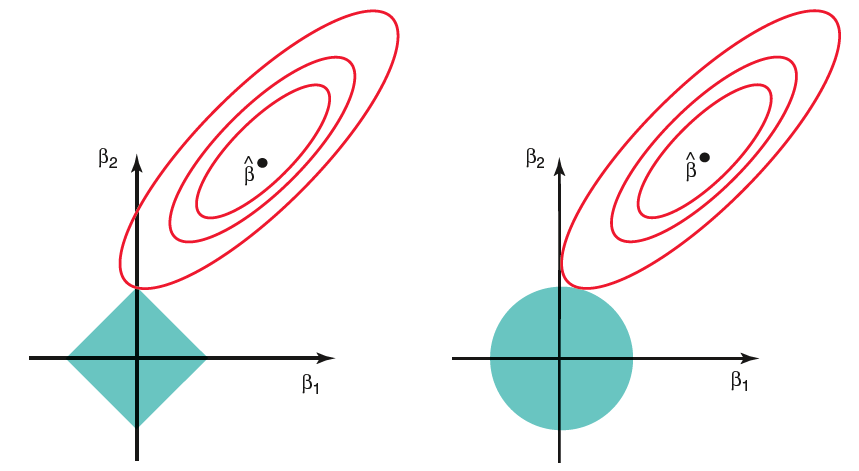
\includegraphics[scale=0.3]{compare.png}
    \caption{}
    \label{}
\end{figure}\end{center}
2维下,Lasso是正方形,Ridge是圆形。\\
- Lasso selects a sub-set of predictors (some coefficients equal to zero).\\
- Ridge regression performs better when the response is a function of many predictors with coefficients around the same size.\\
- Lasso will perform better when a relatively small number of predictors have large coefficients and the rest are very small or equal to zero.\\
- Since the number of predictors is never known a priori, cross-validation can be used to decide which approach is better for a particular data set.

\section{ANOVA: Comparative Experiments}
\subsection{Terminology}
- \textbf{Factor}: an Independent variable. They can be experimental or observational. In our example: Diet\\
- \textbf{Level}: A particular form of the factor. In our example: Levels of the Diet: $A, B, C, D$\\
- \textbf{Treatments}: Factor levels or factor level combinations (if the study contains more than one factors). They provide insights into mechanisms causing the variation being studied. Control treatments?\\
- \textbf{Complete Randomized Design}: Experimental units are randomly split into $r$ groups, and $r$ treatments are assigned, one per group.
\subsection{Data}
$$\begin{array}{ccccc}\text { group } 1 & y_{11}, & y_{12} & \ldots & y_{1 n_{1}} \\ \text { group } 2 & y_{21}, & y_{22} & \ldots & y_{2 n_{2}} \\ \vdots & \vdots & \vdots & \vdots & \vdots \\ \text { group } r & y_{r 1}, & y_{r 2} & \ldots & y_{r n_{r}}\end{array}$$
- $r$ is the number of groups\\
- $n_{i}$ denotes the number of obs in the ith group\\
- $n=\sum_{i=1}^{r} n_{i}$ is the total sample size\\
- $y_{i j}=$ observation $j$ for the ith factor.
\subsection{ANOVA Model}
\subsubsection{ANOVA Means Model}
$$
y_{i j}=\mu_{i}+\varepsilon_{i j}, i=1, \ldots, r ; \quad j=1, \ldots, n_{i}
$$
- $y_{i j}$ : the value of the response in the $j$ th trial for the ith factor.\\
- $\mu_{i}$ : the population mean for the ith factor level (treatment).\\
- $\varepsilon_{i j} \sim^{i i d} \mathcal{N}\left(0, \sigma^{2}\right)$
\subsubsection{Factor Effects Model}
Define the effect of factor level $i$ on the response, i.e. the treatment effect as
$$
\alpha_{i}=\mu_{i}-\mu
$$
where $\mu$ is the overall mean.\\
Factor Effects Model:
$$
\begin{gathered}
y_{i j}=\mu+\alpha_{i}+\varepsilon_{i j}, i=1, \ldots, r ; j=1, \ldots, n_{i} \\
\varepsilon_{i j} \sim^{i i d} \mathcal{N}\left(0, \sigma^{2}\right)
\end{gathered}
$$
- The factor effects model has $r+1$ model parameters, i.e.
$$
\left(\mu, \alpha_{1}, \ldots, \alpha_{r}\right)
$$
- In order for the $\alpha$ 's to be (uniquely) estimated, we need to impose restrictions.\\
- The restrictions on the $\alpha$ 's depend on how $\mu$ is defined.
$$\begin{aligned}
    &\begin{array}{lcc}
    \hline \text { Model } & \mu \text { Definition } & \alpha \text { 's Restriction } \\
    \hline
    \text { Reference Cell } & \mu=\mu_{1} \quad \alpha_{1}=0 \\
    \text { Sum-to-Zero } & \mu=\frac{1}{r} \sum_{i} \mu_{i} & \sum_{i} \alpha_{i}=0 \\
    \text { Weighted Sum-to-Zero } & \mu=\frac{1}{n} \sum_{i} n_{i} \mu_{i} & \sum_{i} n_{i} \alpha_{i}=0 \\
    \hline
    \end{array}\\
    &\text { - The default in } \mathrm{R} \text { is the Reference Cell model. }
\end{aligned}
$$

\subsection{Model Properties}
$\begin{aligned}
&-E\left(y_{i j}\right)=\mu_{i} \\
&-\operatorname{Var}\left(y_{i j}\right)=\operatorname{Var}\left(\varepsilon_{i j}\right)=\sigma^{2}
\end{aligned}$\\
Thus, all observations have the same variance, regardless of factor level.\\
- $\varepsilon_{i j} \sim \mathcal{N}\left(0, \sigma^{2}\right)$ and independent\\
- $y_{i j} \sim \mathcal{N}\left(\mu_{i}, \sigma^{2}\right)$ and independent.\\
We can re-state the model as
\begin{center}
    $y_{i j}$ are independent $\mathcal{N}\left(\mu_{i}, \sigma^{2}\right)$
\end{center}
\subsection{Model Estimation}
Minimize the sum of squared deviations of the observations around their expected values with respect to the parameters:
$$
Q=\sum_{i=1}^{r} \sum_{j=1}^{n_{i}}\left(y_{i j}-\mathbb{E}\left(y_{i j}\right)\right)^{2}
$$
If we re-write $Q$ we have
$$
Q=\sum_{j}\left(y_{1 j}-\mu_{1}\right)^{2}+\sum_{j}\left(y_{2 j}-\mu_{2}\right)^{2}+\ldots+\sum_{j}\left(y_{r j}-\mu_{r}\right)^{2}
$$
So the \textbf{least squares estimator} of $\mu_{i}$, denoted by $\hat{\mu}_{i}$ is
$$
\hat{\mu}_{i}=\bar{y}_{i} .=\frac{1}{n_{i}} \sum_{j=1}^{n_{i}} y_{i j}
$$
Using the appropriate constraints, we can easily extract the estimators for $\mu$ and $\alpha_{i}$.\\
- The $L S$ fit for $y_{i j}$ is the corresponding group mean
$$
\hat{y}_{i j}=\bar{y}_{i}
$$
- Residuals
$$
r_{i j}=y_{i j}-\hat{y}_{i j}=y_{i j}-\bar{y}_{i}
$$
- RSS
$$
\sum_{i=1}^{r} \sum_{j=1}^{n_{i}}\left(y_{i j}-\bar{y}_{i} .\right)^{2}
$$
i.e. the within-group variation.

\begin{equation}
    \begin{array}{cccc}
    \hline
    \text { Source of Variation} & \text { SS } &\text { df } & \text { MS } \\
    \hline \hline \text { Between Groups}& F S S=\sum n_{i}\left(\bar{y}_{i.}-\bar{y}_{..}\right)^{2} & r-1 & \frac{F S S}{r-1} \\
    \text { Error (within Groups)}& R S S=\sum \sum\left(y_{i j}-\bar{y}_{i} .\right)^{2} & n-r & \frac{R S S}{n-r} \\
    \text { Total } & T S S=\sum \sum\left(y_{i j}-\bar{y}_{. .}\right)^{2} & n-1\\
    \hline \hline
    \end{array}
    \nonumber
\end{equation}

\subsection{F-test}
- We want to test whether the means of the groups are really different. We can express this as
$$
\left\{\begin{array}{l}
H_{0}: \mu_{1}=\mu_{2}=\ldots=\mu_{r} \\
H_{\alpha}: \text { not all } \mu_{i}, i=1, \ldots, r \text { are equal }
\end{array}\right.
$$
- or in terms of models
$$
\left\{\begin{array}{l}
H_{0}: y_{i j}=\mu+\varepsilon_{i j} \\
H_{\alpha}: y_{i j}=\mu+\alpha_{i}+\varepsilon_{i j}
\end{array}\right.
$$
- They are two nested models, so we can use the $F$-test
$$
\frac{\left(R S S_{0}-R S S_{\alpha}\right) /(r-1)}{R S S_{\alpha} /(n-r)} \sim F_{r-1, n-r}
$$
under $\mathrm{H}_{0}$.\\
- The test statistic can also be written as
$$
\frac{F S S /(r-1)}{R S S /(n-r)}=\frac{\text { Between-group Variation } /(r-1)}{\text { Within-group Variation } /(n-r)}
$$
where $F S S, R S S$ are defined in the ANOVA table.

\subsection{Diagnostics for ANOVA Models}
– Check for outliers/ unusual observations.\\
– Check the residuals vs. fitted values plot for departures from the constant variance assumption.\\
– Check the Q-Q plot for departures from the normality assumption.\\
\textbf{Levene’s Test} for Equality of Variances:\\
– Run Regression abs(residuals)∼ X, i.e. use abs(residuals) as the response in a new one-way ANOVA.\\
– If the p-value for the F-test is \textbf{greater} than 1\% level, then we conclude that there is no evidence of a non-constant variance.

\subsection{Inference for Factor Level Means ()}













\end{document}